\section{Anharmonic and quantum-crystal corrections}\label{sec:11.5}

At its zero-point amplitude the cubic term of the silicon energy surface is \SI{5}{\percent} of the harmonic one ($\eta_{\mathrm{anh}} = 0.049$, \cref{sec:5.7}), and every formula of \cref{sec:11.3,sec:11.4} dropped it. How much does that change a rate? For the impulse peak, by a part in a thousand. For a deposit of several phonons at a momentum transfer of a few keV, by factors of several, because an anharmonic lattice can make many phonons out of one kick, which a harmonic lattice can only do with many kicks. In solid helium the zero-point motion of an atom is a quarter of the distance to its neighbor, and some harmonic frequencies are imaginary. And in a crystal with a soft mode or a light atom no expansion is available at all, and only exact moments of the response, which anharmonicity cannot change, bound it.

\subsection{Exact moments of the self response}

Above a few zone momenta each nucleus responds on its own (\cref{sec:11.3}), and its self response is controlled by the kick operator $D = E_R + \vect{q}\cdot\vect{p}/M_\kappa$ of \cref{sec:11.4}: the Hamiltonian after the kick is $H + D$, exactly, whatever the potential, provided it depends on the positions of the nuclei and not on their momenta (\cref{eq:D.32-I}). Normalize the response to a distribution in $\omega$, $\dd P = S\,\dd\omega/\int S\,\dd\omega$, with moments $\mu_k = \int\omega^k\,\dd P$ and central moments $\bar\mu_k$, as in \cref{app:C.10}. At $T = 0$, writing $A = H - E_0$, which annihilates the ground state, and $\delta D = D - E_R = (q/M_\kappa)p_{\hat q}$, the central moments are $\bar\mu_k = \langle(A + \delta D)^k\rangle$. Every term with $A$ at either end vanishes. The zeroth moment is $\mu_0 = 1$: the weight of the self response is the norm of $\ee^{\ii\vect{q}\cdot\vect{X}}|0\rangle$. The first is $\mu_1 = E_R$, the sum rule \cref{eq:5.6-sum}. The second and third were derived in \cref{app:D.32}. The fourth needs one more step: of the four terms of $\langle\delta D(A + \delta D)^2\delta D\rangle$, the term $\langle\delta D\,A^2\,\delta D\rangle$ is the squared norm of $A\,\delta D|0\rangle = [H, \delta D]|0\rangle$, and $[H, p_{\hat q}] = \ii\,\partial_{\hat q}V$ is the force along $\hat{\vect{q}}$. The two mixed terms $\langle\delta D\,A\,\delta D^2\rangle$ and its complex conjugate equal $\ii(q/M_\kappa)^3\langle p_{\hat q}(p_{\hat q}\partial_{\hat q}V + \partial_{\hat q}V\,p_{\hat q})\rangle$, by $[H, p_{\hat q}^2] = \ii(p_{\hat q}\partial_{\hat q}V + \partial_{\hat q}V\,p_{\hat q})$; for a real ground-state wavefunction the average is real, so the term is imaginary and cancels against its conjugate. Collecting,
\begin{keyresult}[Exact moments of the self response]
\begin{equation}
  \begin{gathered}
  \mu_0 = 1 , \qquad \mu_1 = E_R , \qquad
  \bar\mu_2 = 4E_RE^{\mathrm{kin}}_\kappa , \\
  \bar\mu_3 = \frac{q^2}{2M_\kappa^2}\bigl\langle\partial_{\hat q}^2V\bigr\rangle , \quad
  \bar\mu_4 = \frac{q^2}{M_\kappa^2}\bigl\langle(\partial_{\hat q}V)^2\bigr\rangle + \frac{q^4}{M_\kappa^4}\bigl\langle p_{\hat q}^4\bigr\rangle ,
  \end{gathered}
  \label{eq:11.5-moments}
\end{equation}
for any potential $V$ of the nuclei, with $E^{\mathrm{kin}}_\kappa = \langle p_{\hat q}^2\rangle/2M_\kappa$ the kinetic energy along $\hat{\vect{q}}$ of \cref{eq:11.4-width}. The averages are over the ground state at $T = 0$; all five moments hold at any temperature with thermal averages (\cref{app:D.32}).
\end{keyresult}
\noindent Each moment is an equal-time average in the ground state: the kinetic energy, the mean curvature of the energy surface, the mean-square force and the fourth moment of the momentum distribution. For a harmonic crystal they reproduce the cumulants of \cref{eq:D.32-ck}; for one oscillator of frequency $\omega_0$, for instance, the mean-square force is $M_\kappa^2\omega_0^4\langle u_{\hat q}^2\rangle = M_\kappa\omega_0^3/2$, so the first term of $\bar\mu_4$ is the fourth cumulant $E_R\omega_0^3$, and the second is $3\bar\mu_2^2$. In an anharmonic crystal the same averages come from a path-integral simulation of the nuclei, which needs no dynamics (\cref{app:E.19}). They are the self part of the moments $\mathscr{M}^k$ of \cref{eq:8.3-moments} for one species, divided by $\mathscr{M}^0$.

Write its relative correction to the harmonic self response as $\delta_{\mathrm{anh}}(\vect{q},\omega) = S_A/S_A^{\mathrm{harm}} - 1$. Then the weight $\int S_A^{\mathrm{harm}}\delta_{\mathrm{anh}}\,\dd\omega$ and the first moment $\int\omega\,S_A^{\mathrm{harm}}\delta_{\mathrm{anh}}\,\dd\omega$ vanish exactly, and the second moment $\int\omega^2S_A^{\mathrm{harm}}\delta_{\mathrm{anh}}\,\dd\omega$ is fixed by the change of the kinetic energy, $4E_R(E^{\mathrm{kin}}_\kappa - E^{\mathrm{kin,harm}}_\kappa)$ times the weight. These three linear constraints test any calculation of the anharmonic response. Time reversal adds a selection rule. For a target invariant under time reversal the eigenfunctions are real, $|\langle f|\ee^{\ii\vect{q}\cdot\vect{X}}|0\rangle|^2 = |\langle f|\ee^{-\ii\vect{q}\cdot\vect{X}}|0\rangle|^2$, and the response is even in $\vect{q}$. A term of first order in $\Phi^{(3)}$ carries three displacements from the cubic term of \cref{eq:5.7-H3}, so it needs an odd number of displacements from the kick to pair them all, and it is odd in $\vect{q}$. It therefore vanishes. The first anharmonic correction to the rate is of second order in $\Phi^{(3)}$ and first order in $\Phi^{(4)}$, the level $n_A = 2$ of \cref{sec:8.5}, of relative size $\eta_{\mathrm{anh}}^2$ by \cref{eq:5.7-order}.

\subsection{Cubic phonon decay}

In the impulse regime the first correction is small. The impulse response \cref{eq:11.4-IA} depends on the potential only through the momentum distribution $\mathfrak{f}_\kappa$, and its width through $E^{\mathrm{kin}}_\kappa$. A single-site model holds the neighbors of one nucleus fixed and gives it a one-dimensional anharmonic potential~\cite[Eq.~(26)]{lin2024anharmonic},
\begin{equation}
  V(x) = \tfrac12M_\kappa\omega_0^2x^2 + \lambda_3\,\omega_0\Bigl(\frac{x}{\ell_0}\Bigr)^3 + \lambda_4\,\omega_0\Bigl(\frac{x}{\ell_0}\Bigr)^4 , \qquad \ell_0 = (2M_\kappa\omega_0)^{-1/2} ,
  \label{eq:11.5-toy}
\end{equation}
with $\ell_0$ the zero-point amplitude of the oscillator. In this potential the cubic energy at $x = \ell_0$ is $4\lambda_3$ times the harmonic one, and $4\lambda_3$ is the anharmonic parameter of \cref{eq:5.7-eta} measured on the site coordinate instead of the bond. Fits of an empirical silicon potential along the bond and perpendicular to it give $\lambda_3 = 0.006$ to $0.01$ and $\lambda_4 = (2$ to $3)\times10^{-4}$~\cite[Sect.~IV]{lin2024anharmonic}, so $4\lambda_3 = 0.024$ to $0.04$, of the size of the bond value $0.049$ of \cref{sec:5.7}. To second order in $\lambda_3$ and first in $\lambda_4$ the kinetic energy becomes $E^{\mathrm{kin}} = (\omega_0/4)(1 - 44\lambda_3^2 + 12\lambda_4)$~\cite[Eq.~(65)]{lin2024anharmonic}, a change within $\pm\SI{0.2}{\percent}$ over the silicon ranges of $\lambda_3$ and $\lambda_4$. The impulse width $\sigma_\omega \propto (E^{\mathrm{kin}})^{1/2}$ then moves by at most a part in a thousand, \SI{0.09}{meV} of the \SI{88}{meV} of \cref{we:11-width}.

At smaller $q$ the correction is of a different kind, because anharmonicity changes how many kicks a given number of phonons needs. Expand the self response of \cref{eq:11.3-exact} in powers of $q$. At $\omega \neq 0$ the constant and the averages of single displacements contribute only at $\omega = 0$, and the first term is the correlation of two displacements,
\begin{equation*}
  S_A(\vect{q},\omega) = \frac{1}{\Omega}\sum_\kappa c_\kappa^2\,q_\alpha q_\beta\int\dd t\;\ee^{\ii\omega t}\bigl\langle u^\alpha_{\kappa}(t)\,u^\beta_{\kappa}(0)\bigr\rangle + O(q^4) ,
\end{equation*}
exact for any anharmonicity. Insert the displacement in phonon coordinates, $\vect{u}_{\vect{R}\kappa} = \sum_{\vect{Q}\nu}(2NM_\kappa\omega_{\vect{Q}\nu})^{-1/2}\vect{e}_{\kappa\nu}(\vect{Q})\ee^{\ii\vect{Q}\cdot\vect{R}}B_{\vect{Q}\nu}$ (\cref{sec:5.3}). The correlation of $B_{\vect{Q}\nu}$ is the spectral function of the dressed propagator $\mathsf{D}_\nu(\vect{Q},\omega) = 2\omega_{\vect{Q}\nu}/[\omega^2 - \omega_{\vect{Q}\nu}^2 - \Pi_\nu(\vect{Q},\omega)]$ of \cref{eq:6.4-Pi}: at $T = 0$ and $\omega > 0$, $\int\dd t\,\ee^{\ii\omega t}\langle B_{\vect{Q}\nu}(t)B_{-\vect{Q}\nu}\rangle = -2\Imag\mathsf{D}_\nu(\vect{Q},\omega)$, which is $2\pi\delta(\omega - \omega_{\vect{Q}\nu})$ for the free phonon. Here $\Pi_\nu$ is the anharmonic self-energy: the bubble of two cubic vertices of \cref{eq:5.7-V3}, whose imaginary part on shell is $-\omega_{\vect{Q}\nu}\gamma^{\mathrm{anh}}_{\vect{Q}\nu}$ (\cref{eq:5.7-gamma,eq:6.4-pole}), and the loop of one quartic vertex, which is real. Off shell, $-\Imag\Pi_\nu(\vect{Q},\omega) = \omega_{\vect{Q}\nu}\gamma^{\mathrm{anh}}_{\vect{Q}\nu}(\omega)$, with $\gamma^{\mathrm{anh}}_{\vect{Q}\nu}(\omega)$ the width of \cref{eq:5.7-gamma} with the energy $\omega$ in place of $\omega_{\vect{Q}\nu}$ in the delta function of the decay: the rate at which a phonon of momentum $\vect{Q}$, given the energy $\omega$, decays into two. With the branches kept separate, as in \cref{sec:6.4}, the harmonic term gives back the one-phonon response \cref{eq:11.1-S1}, a delta function on each branch. Away from the poles, above the one-phonon band, the first order in $\Pi_\nu$ is $-\Imag\mathsf{D}_\nu = 2\omega_{\vect{Q}\nu}(-\Imag\Pi_\nu)/(\omega^2 - \omega_{\vect{Q}\nu}^2)^2$, and
\begin{keyresult}[First anharmonic correction to the nuclear response]
\begin{equation}
  S_A^{\mathrm{anh}}(\vect{q},\omega) = \frac{2\pi}{\Omega}\sum_\kappa c_\kappa^2\,\ee^{-2W_\kappa}\,\frac1N\sum_{\vect{Q}\nu}\frac{|\vect{q}\cdot\vect{e}_{\kappa\nu}(\vect{Q})|^2}{\pi M_\kappa}\;
  \frac{\omega_{\vect{Q}\nu}\,\gamma^{\mathrm{anh}}_{\vect{Q}\nu}(\omega)}{(\omega^2 - \omega_{\vect{Q}\nu}^2)^2} ,
  \label{eq:11.5-anh}
\end{equation}
at $T = 0$, for $\omega$ outside the one-phonon band and $q$ above a few $q_{\mathrm{BZ}}$, where the self part is the response. It is of order $q^2$ and of second order in $\Phi^{(3)}$; the Debye--Waller factor, which the higher orders in $q$ supply, is written to leading order in $\eta_{\mathrm{anh}}$.
\end{keyresult}
\noindent The physical picture is that of \cref{fig:6-bubble} with the electron bubble replaced by a pair of phonons: the kick creates one phonon off its energy shell, and it decays into two real ones. Near $\omega = \omega_{\vect{Q}\nu}$ the same expression, resummed, is the Lorentzian tail of a phonon line of full width $\gamma^{\mathrm{anh}}_{\vect{Q}\nu}$. The two time orderings, the decay of a virtual phonon and the creation of three from the vacuum, have the denominators $1/(\omega - \omega_{\vect{Q}\nu})$ and $1/(\omega + \omega_{\vect{Q}\nu})$, which combine into the $2\omega_{\vect{Q}\nu}/(\omega^2 - \omega_{\vect{Q}\nu}^2)$ of $\mathsf{D}_\nu$.

How large is \cref{eq:11.5-anh} against the harmonic two-phonon response? The harmonic term needs two kicks and carries $q^4$; the anharmonic term needs one kick and the factor $\gamma^{\mathrm{anh}}/\omega \sim \eta_{\mathrm{anh}}^2$. Their ratio is $\sim\eta_{\mathrm{anh}}^2\,2M_\kappa\omega/q^2$, large at small $q$. The model \cref{eq:11.5-toy} makes the counting exact. To first order in $\lambda_3$, with $x/\ell_0 = a + a^\dagger$ and the harmonic states $|n\rangle$ in units of $\omega_0$, the ground state and the second level become
\begin{equation*}
  |\tilde0\rangle = |0\rangle - \lambda_3\Bigl(3|1\rangle + \sqrt{\tfrac23}\,|3\rangle\Bigr) , \qquad
  |\tilde2\rangle = |2\rangle + 6\sqrt2\,\lambda_3|1\rangle + \dots ,
\end{equation*}
where the dots stand for $|3\rangle$ and $|5\rangle$, which the kick does not connect to $|\tilde0\rangle$ at first order in $q$. The coefficient $6\sqrt2$ is $\langle1|(a + a^\dagger)^3|2\rangle$ divided by the level spacing. With $k = q\ell_0$ the kick is $\ee^{\ii k(a + a^\dagger)} = 1 + \ii k(a + a^\dagger) - \frac12k^2(a + a^\dagger)^2 + \dots$. The constant term vanishes between orthogonal states. The linear term gives $\langle\tilde2|a + a^\dagger|\tilde0\rangle = -\lambda_3(3\sqrt2 + \sqrt2) + 6\sqrt2\,\lambda_3 = 2\sqrt2\,\lambda_3$. The quadratic term gives the harmonic $-k^2/\sqrt2$. One amplitude is imaginary and the other real; they do not interfere, and the weight of the second level is
\begin{equation}
  |\langle\tilde2|\ee^{\ii qx}|\tilde0\rangle|^2 = \ee^{-k^2}\Bigl(\frac{k^4}{2} + 8\lambda_3^2k^2 + \dots\Bigr) , \qquad
  \frac{\text{anharmonic}}{\text{harmonic}} = \frac{16\lambda_3^2}{k^2} ,
  \label{eq:11.5-two}
\end{equation}
The anharmonic term wins below $k = 4\lambda_3$, that is, below $q_\times = 4\lambda_3(2M_\kappa\omega_0)^{1/2}$: the crossover sits where the momentum transfer, in units of the inverse zero-point amplitude, equals the anharmonic parameter. For silicon, with $\omega_0 = \langle\omega^{-1}\rangle^{-1} = \SI{30.4}{meV}$, $(2M_\kappa\omega_0)^{1/2} = \SI{39.9}{keV}$ and $q_\times = \SI{1.6}{keV}$ for $\lambda_3 = 0.01$, just below $q_{\mathrm{BZ}} = \SI{2.25}{keV}$. At $q_{\mathrm{BZ}}$ the two-phonon weight is raised by \SI{50}{\percent} for $\lambda_3 = 0.01$ and by \SI{18}{\percent} for $0.006$.

More phonons need more kicks, and the anharmonic gain grows with their number. Three phonons need three kicks in the harmonic crystal, $k^6/6$, but only two with one cubic vertex. That two-kick amplitude alone gives $24\lambda_3^2k^4$; interference between the one-kick amplitude of order $\lambda_3^2k$ and the harmonic three-kick amplitude $k^3/\sqrt6$ subtracts $6\lambda_3^2k^4$, for a net $18\lambda_3^2k^4$. The ratio is then $108\lambda_3^2/k^2$ and the crossover lies at $k = 10.4\lambda_3$, \SI{4.2}{keV} for $\lambda_3 = 0.01$. In general an $n$-phonon weight acquires terms $\lambda_3^{j}k^{2i}$ with $i < n$, and the smaller $i$ the higher the power $j$~\cite[Eqs.~(39), (45)--(48)]{lin2024anharmonic}. \Cref{lim:11.5a} shows the result: for $\lambda_3 = 0.01$ the harmonic two-, three- and four-phonon weights hold within \SI{10}{\percent} only above 5, 12 and \SI{20}{keV}, while at $q_{\mathrm{BZ}}$ the four-phonon weight is 27 times the harmonic one. Which rates does this affect? A threshold of $\omega_{\mathrm{th}}$ needs at least $\omega_{\mathrm{th}}/\omega_{\mathrm{max}}$ phonons, and a particle of mass $\mchi$ reaches at most $q = 2\mchi v_{\mathrm{max}}$. High thresholds and masses of a few MeV are therefore where the harmonic multiphonon rate fails. In the single-site model the anharmonic rate exceeds the harmonic one by up to two orders of magnitude for masses of a few MeV and thresholds of a few phonon energies, in the tail of the spectrum where the rate is small, and the two agree above \SI{10}{MeV}~\cite[Sect.~IV\,A]{lin2024anharmonic}. The anharmonic rate is never below the harmonic one there, because the term of lowest order in $q$ is a square, $|\langle f|\ii qx|\tilde0\rangle|^2$, which the harmonic crystal lacks for $n \ge 2$; this holds for the leading term, not for the full response.

\begin{limitbox}[Anharmonic corrections to multiphonon weights][lim:11.5a]
For a nucleus in the potential \cref{eq:11.5-toy}, the $n$-phonon weight carries, besides the harmonic $\ee^{-k^2}k^{2n}/n!$, terms $\lambda_3^jk^{2i}$ with $i < n$, which dominate for small $k = q\ell_0$; the kinetic energy changes as $1 - 44\lambda_3^2 + 12\lambda_4$~\cite[Eqs.~(39), (45)--(48), (65)]{lin2024anharmonic}.
\par\smallskip
{\centering
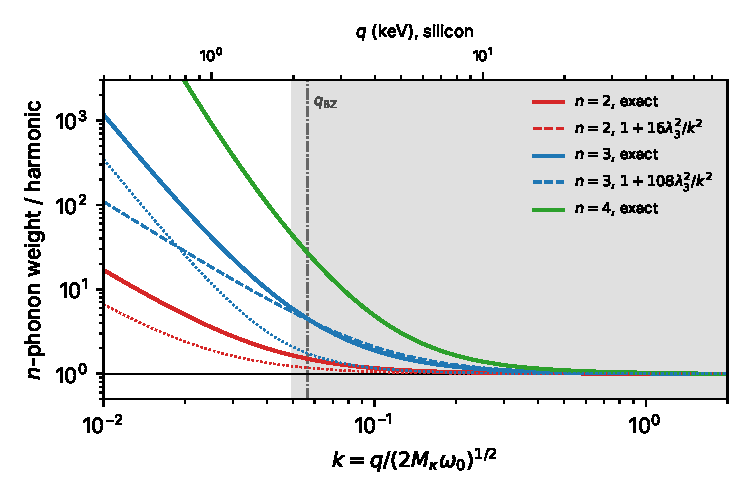
\includegraphics[width=\linewidth]{figures/ch11/limit11_5a.pdf}
\captionof{figure}{Weight of the $n$-th level of the single-site model \cref{eq:11.5-toy}, divided by the harmonic Poisson weight $\ee^{-k^2}k^{2n}/n!$, against $k = q/(2M_\kappa\omega_0)^{1/2}$, for $n = 2$ (red), 3 (blue) and 4 (green). Model with the silicon values $\omega_0 = \SI{30.4}{meV}$, $M_\kappa = \SI{26.16}{GeV}$, $\lambda_3 = 0.01$, $\lambda_4 = 2.5\times10^{-4}$ (solid), and $\lambda_3 = 0.006$, $\lambda_4 = 2\times10^{-4}$ (dotted), solved exactly in 200 oscillator states. Dashed: the leading anharmonic terms, $1 + 16\lambda_3^2/k^2$ for $n = 2$ (\cref{eq:11.5-two}) and $1 + 108\lambda_3^2/k^2$ for $n = 3$. Dash-dotted: $q_{\mathrm{BZ}} = \SI{2.25}{keV}$. Gray band: $k \ge 0.05$, where both leading terms are within \SI{10}{\percent} of the exact weights; below it the three-phonon weight is dominated by a term of order $\lambda_3^4k^2$.}\label{fig:11-limit-5a}
\par}
\smallskip
The model fixes the neighbors, so it overstates the effect below $q_{\mathrm{BZ}}$, where translation invariance makes every multiphonon term of a mass-proportional coupling of order $q^4$; at large $k$ the weights return to the harmonic ones.
\end{limitbox}

\noindent The single-site model breaks translation invariance: a nucleus pulled against fixed neighbors feels a force even when the whole crystal moves. In the real crystal the soft acoustic limit \cref{eq:8.3-soft} is exact, anharmonic terms included, and for a coupling proportional to mass every response at fixed $\omega \neq 0$ vanishes as $q^4$ for $q \ll q_{\mathrm{BZ}}$. The term of order $q^2$ in \cref{eq:11.5-anh} survives because, above $q_{\mathrm{BZ}}$, the self part no longer cancels against the distinct part. Below $q_{\mathrm{BZ}}$ the anharmonic two-phonon response has the same $q^4$ as the harmonic one, and in GaAs it dominates the harmonic term near the on-shell longitudinal-acoustic resonance, where that resonance is kinematically accessible~\cite[Fig.~2]{campbelldeem2020multiphonon}. The window in which the anharmonic $q^2$ term dominates is therefore $q_{\mathrm{BZ}} \lesssim q \lesssim q_\times(n)$, open for three and more phonons in silicon and germanium.

On the truncation label of \cref{sec:8.5}, \cref{eq:11.5-anh} is the first correction along the anharmonic axis, $n_A = 2$, with $\mathcal{K}$ = multiphonon, $n_B = 0$ and $n_T = 0$; at finite temperature the factor $1 + n_B(\omega)$ multiplies it and the thermal factors of \cref{eq:5.7-gamma} enter $\gamma^{\mathrm{anh}}$. The self-energy needs the cubic force constants of the whole crystal on a grid of $\vect{Q}$, which density-functional perturbation theory or finite displacements in a supercell provide (\cref{sec:5.4,app:E.8}). No such calculation exists yet; the single-site model is the only estimate.

\subsection{The Markov--Krein band}

Perturbation theory in $\Phi^{(3)}$ fails for soft modes, light atoms and quantum crystals, but the moments \cref{eq:11.5-moments} do not need it. They are static averages, computable for any anharmonicity, and \cref{app:C.10} shows how much five moments say about a distribution. Every distribution with the moments $\mu_0, \dots, \mu_4$ has its cumulative $F(\xi) = \int_{-\infty}^{\xi}\dd P$ inside the Markov--Krein band \cref{eq:C.10-band}. At each $\xi$ the band is spanned by the canonical representation through $\xi$: three point masses $w_i$ at $y_i$, one of them at $\xi$, that reproduce the five moments, $\sum_iw_iy_i^k = \mu_k$ for $k = 0, \dots, 4$. These are five equations for the two free positions and the three weights. The weight below $\xi$ and the weight up to and including $\xi$ bound $F(\xi)$ from below and above. The width of the band is the mass at $\xi$, the largest that any distribution with these moments can put there: the Christoffel function $\varrho_{\mathrm{MK}}(\xi)$ of \cref{eq:C.10-rho}. For a Gaussian the width is $2/(3 + \xi^4)$, with $\xi$ in standard deviations from the mean (\cref{eq:C.10-gauss}).

\Cref{fig:11-mk} draws the band around the harmonic response of silicon at $q = \SI{100}{keV}$, the momentum of \cref{we:11-width}, and at \SI{50}{keV}. The moments are those of the cumulants $c_k = E_R\langle\omega^{k-1}\rangle$ of \cref{eq:D.32-ck}, which the numerical spectrum reproduces to $10^{-6}$ at \SI{100}{keV}. The response lies inside the band everywhere, as it must. Near the peak the band is wide (\cref{we:11-mkpeak}); at \SI{50}{keV}, where the zero-phonon line puts a step of 0.21 at $\omega = 0$ and the phonon bands show, it spans 0.21 to 0.89 at $\omega = E_R$. In the tails it narrows as $(\xi - \mu_1)^{-4}$, with the coefficient $\bar\mu_4 - \bar\mu_2^2 - \bar\mu_3^2/\bar\mu_2$ of \cref{eq:C.10-tail}.

\begin{figure}[tbp]
  \centering
  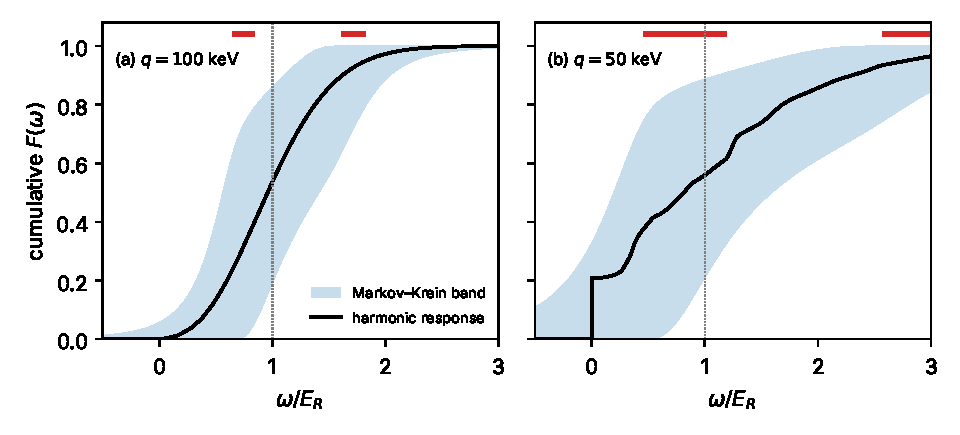
\includegraphics[width=\linewidth]{figures/ch11/fig11_5.pdf}
  \caption{Cumulative nuclear response $F(\omega)$ of silicon at $T = 0$ (black), the fraction of the weight of the self response at energies up to $\omega$, against $\omega/E_R$, with the Markov--Krein band of its first five moments (blue). (a)~$q = \SI{100}{keV}$, $E_R = \SI{191.1}{meV}$, $x_R = 4.67$; (b)~$q = \SI{50}{keV}$, $E_R = \SI{47.8}{meV}$, $x_R = 1.17$, where the zero-phonon weight $\ee^{-2W_\kappa} = 0.21$ is a step at $\omega = 0$. Response: harmonic, incoherent, all phonon orders, from the PBE density of states of \cref{sec:5.2}; moments from $c_k = E_R\langle\omega^{k-1}\rangle$. Red bars: values of $\omega$ at which a node of the canonical representation lies below $\omega = 0$, so that the band drawn is wider than the sharp band of distributions confined to $\omega \ge 0$; elsewhere it is sharp for them too. Dotted: $\omega = E_R$.}
  \label{fig:11-mk}
\end{figure}

At $T = 0$ the response vanishes for $\omega < 0$, a constraint that the band of \cref{eq:C.10-band} does not use. It remains valid, and where every node of the canonical representation lies at $\omega \ge 0$ that representation is itself an admissible response, which makes the band sharp on the half line too. This holds at $\omega = E_R$ for $q = \SI{100}{keV}$ (\cref{we:11-mkpeak}). It fails in two windows, $0.65$ to $0.85\,E_R$ and $1.61$ to $1.82\,E_R$, where one outer node of the three-point solution moves out to infinity and comes back from the other side, below $\omega = 0$; at \SI{50}{keV} the windows are $0.46$ to $1.20\,E_R$ and $2.6$ to $3.4\,E_R$. There the half-line point-mass bound \cref{eq:C.10-stieltjes} is smaller than $\varrho_{\mathrm{MK}}$, by up to \SI{6.8}{\percent} at \SI{100}{keV} and \SI{24.5}{\percent} at \SI{50}{keV}, so the sharp half-line band is narrower at least by that much. We use the band \cref{eq:C.10-band} throughout, which is conservative and has explicit extremal distributions.

\begin{workedexample}{Markov--Krein band of silicon at the recoil energy}\label{we:11-mkpeak}
Take silicon at $q = \SI{100}{keV}$ and $T = 0$, with $E_R = \SI{191.1}{meV}$ and $\langle\omega\rangle = \SI{40.9}{meV}$ as in \cref{we:11-width}. The cumulants $c_k = E_R\langle\omega^{k-1}\rangle$ give the standard deviation $\sigma_\omega = \SI{88.4}{meV}$, the skewness $c_3/\sigma_\omega^3 = 0.553$ and the standardized fourth moment $3 + c_4/c_2^2 = 3 + (\langle\omega^3\rangle/\langle\omega\rangle^3)/x_R = 3.333$, against 0 and 3 for a Gaussian. For a Gaussian the canonical representation through the mean has nodes at 0 and $\pm\sqrt3$ standard deviations with weights $\tfrac23, \tfrac16, \tfrac16$ (\cref{app:C.10}). For silicon the same construction, \cref{eq:C.10-kernel} with these moments, puts the nodes at 59.8, 191.1 and \SI{371.3}{meV} with weights 0.191, 0.670 and 0.139. The skewness pushes the outer nodes upward and moves weight to the lower one, but leaves the central weight at $\varrho_{\mathrm{MK}}(E_R) = 0.670$, almost the Gaussian 2/3. So
\begin{equation*}
  0.191 \le F(E_R) \le 0.861 ,
\end{equation*}
while the harmonic response has $F(E_R) = 0.537$. A detector with its threshold at $E_R$ sees between 14 and \SI{81}{\percent} of the events of this momentum transfer, whatever the dynamics, if only the five moments are right.

Energy bins narrow the band little. Between $E_R - \sigma_\omega$ and $E_R + \sigma_\omega$ the band allows any weight from 0.07 to 1.00 (the harmonic value is 0.68); between $E_R \pm 2\sigma_\omega$ it allows 0.78 to 1.00 (0.96). In the tail it is worse in relative terms: above $E_R + 3\sigma_\omega = \SI{456}{meV}$ the harmonic response has the weight $5.6\times10^{-3}$, and the band allows anything from 0 to $3.4\times10^{-2}$, six times more.

The anharmonic change of the kinetic energy of silicon moves the cumulative distribution by at most $2.5\times10^{-4}$, nearly three thousand times less than the width of the band at the peak. For silicon the perturbative correction of the previous subsection is the tool; the band is for targets where no correction can be computed.
\end{workedexample}

In silicon at \SI{100}{keV} the band fixes the weight above a threshold to \SI{10}{\percent} only for thresholds at $\omega \le \SI{28}{meV}$ (\cref{lim:11.5c}). At five standard deviations above the mean the band is 63 times the weight.

\begin{limitbox}[The Markov--Krein band][lim:11.5c]
Every distribution with the moments $\mu_0, \dots, \mu_4$ has $\sum_{y_i < \xi}w_i \le F(\xi) \le \sum_{y_i \le \xi}w_i$, of width $\varrho_{\mathrm{MK}}(\xi)$, with $(y_i, w_i)$ the canonical representation through $\xi$; far from the mean $\varrho_{\mathrm{MK}} \simeq (\bar\mu_4 - \bar\mu_2^2 - \bar\mu_3^2/\bar\mu_2)/(\xi - \mu_1)^4$~\cites{krein1977markov}{akhiezer1965classical}.
\par\smallskip
{\centering
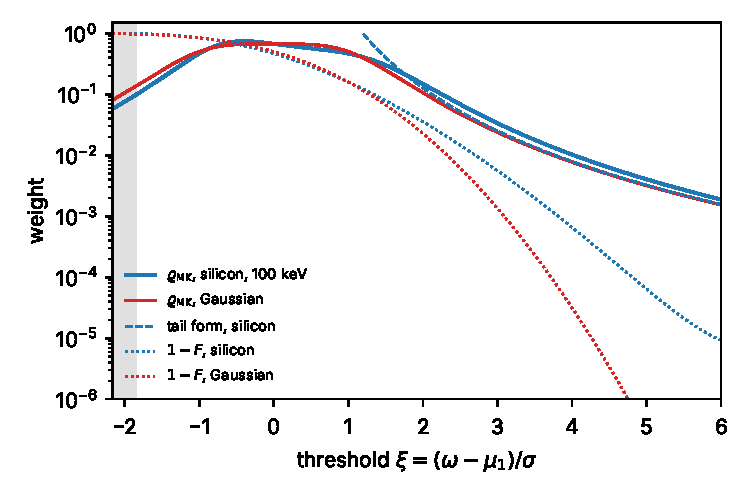
\includegraphics[width=\linewidth]{figures/ch11/limit11_5c.pdf}
\captionof{figure}{Width $\varrho_{\mathrm{MK}}$ of the band (solid) and weight $1 - F$ above a threshold (dotted), against the threshold $\xi$ in units of the standard deviation from the mean, for the harmonic silicon response at $q = \SI{100}{keV}$ (blue; skewness 0.553, standardized fourth moment 3.333) and for a Gaussian (red), the two model distributions whose five moments define their bands. Dashed: the tail form \cref{eq:C.10-tail} for silicon, the leading term far from the mean, with the numerator 2.03 (2 for the Gaussian); the exact width exceeds it by \SI{34}{\percent} at $\xi = 3$ and \SI{20}{\percent} at $\xi = 6$, a correction of relative order $1/\xi$ from the skewness. The silicon curves start at $\omega = 0$. Gray band: thresholds at which the band fixes the silicon weight above threshold to \SI{10}{\percent}, $\varrho_{\mathrm{MK}} \le 0.1\,(1 - F)$, that is $\xi \le -1.84$.}\label{fig:11-limit-5c}
\par}
\smallskip
Above about two standard deviations below the mean the absolute width exceeds a tenth of the weight above threshold, and in the tail it exceeds the weight itself: the band bounds the bulk of a response, never the ratio of two tails.
\end{limitbox}

\noindent On the truncation label the band is exact in $n_A$ and in $n_T$ when the moments are, and it makes no assumption about $\mathcal{K}$. Its use is twofold. For a strongly anharmonic target at a detector temperature it is the only rigorous statement about the response, since the moments come from a static simulation and every real-time method has a problem at millikelvin (below). And for any approximate dynamics it is an acceptance test: a computed response outside the band of its exact moments is wrong.

\subsection{Solid helium}

Helium solidifies only under a pressure of a few MPa even at the lowest temperatures~\cite{ashour2024pressure}, because the zero-point energy of so light an atom in so shallow a well, \SI{10.8}{K} deep for a pair~\cite{aziz1979accurate}, competes with the binding itself. Such a solid is a \emph{quantum crystal}: the zero-point amplitude of an atom is a sizable fraction of the distance to its neighbors, about a quarter near melting, and the harmonic expansion fails at its lowest order. The Lindemann ratio $r_{\mathrm{L}} = \langle u^2\rangle^{1/2}/d_{\mathrm{nn}}$, the root-mean-square displacement over the nearest-neighbor distance $d_{\mathrm{nn}}$, measures it. At the static lattice positions an atom sits far out on the attractive tail of its neighbors' potentials, where the curvature is negative, and the static force constants give imaginary frequencies. The self-consistent harmonic approximation of \cref{eq:5.7-scha} was devised for this case: averaged over the Gaussian spread of the atom, the curvature includes the steep repulsion that the atom samples on its excursions, and it is positive. Compression reduces $r_{\mathrm{L}}$. Diffusion Monte Carlo calculations with a pair potential fitted to dispersion-corrected density-functional theory find $r_{\mathrm{L}} = 0.12$ at \SI{2}{GPa} and 0.10 from \SI{14}{GPa} up to \SI{150}{GPa}~\cite[Table~I]{cazorla2015first}. At such pressures the static lattice is stable, and the quasi-harmonic approximation of \cref{sec:5.7} becomes a reasonable starting point.

Ashour and Griffin proposed solid helium under pressure as a target for light dark matter that couples to nucleons~\cite{ashour2024pressure}. At low pressure its phonon energies are below \SI{3}{meV} and its sound speed is of order $10^{-6}$, too low for single-phonon reach. Between 1 and \SI{40}{GPa} the sound speed rises more than tenfold and the phonon energies nearly a hundredfold, and at \SI{40}{GPa} the single-phonon reach of hcp helium rivals that of diamond. Their response is that of \cref{lim:11.5b}, with phonons computed with the PBE functional and a dispersion correction, and it leaves out the low pressures, where the density functional fails and the Born--Oppenheimer phonons miss the zero-point motion.

When is the quasi-harmonic response good enough, and what does the self-consistent one add? \Cref{lim:11.5b} answers in a cell model, in which one atom moves in the field of its twelve neighbors held fixed on an fcc lattice and the Schrödinger equation is solved exactly. The pair potential is a Morse form with the well of the helium potential, so that only one shape parameter is chosen (the curvature at the minimum of a 12-6 potential with the same well). The model gives $r_{\mathrm{L}} = 0.23$ at \SI{21}{cm^3.mol^{-1}}, near melting, where its first excitation lies at \SI{2.2}{meV}, and 0.117 and 0.094 at the volumes of the Monte Carlo values 0.12 and 0.10 above. The static curvature turns negative for molar volumes above \SI{17}{cm^3.mol^{-1}}, $r_{\mathrm{L}} \ge 0.20$. Below that the quasi-harmonic weight of a single phonon, $q^2/2M\omega$ per direction, overshoots the exact one, because the static curvature is too soft; the error falls below \SI{10}{\percent} only for $r_{\mathrm{L}} \le 0.115$, a molar volume of \SI{6.5}{cm^3.mol^{-1}}, about the \SI{2}{GPa} of the Monte Carlo calculation. The self-consistent harmonic weight stays within \SI{10}{\percent} up to $r_{\mathrm{L}} = 0.227$ and is \SI{10}{\percent} low at \SI{21}{cm^3.mol^{-1}}. The kinetic energy that sets the impulse width behaves alike: at $r_{\mathrm{L}} = 0.117$ the quasi-harmonic value is \SI{9}{\percent} low and the self-consistent one within \SI{0.1}{\percent}.

\begin{limitbox}[Solid helium: quasi-harmonic and self-consistent phonons][lim:11.5b]
The single-phonon rate of compressed helium is \cref{eq:11.1-S1} with $c_\kappa = A_\kappa F_N$, phonons and Debye--Waller exponent from the static Hessian at the compressed volume~\cite[Eqs.~(2), (4), (5)]{ashour2024pressure}; the self-consistent correction replaces the Hessian by $\Phi^{(2)}_{\mathrm{aux}}$ of \cref{eq:5.7-scha}.
\par\smallskip
{\centering
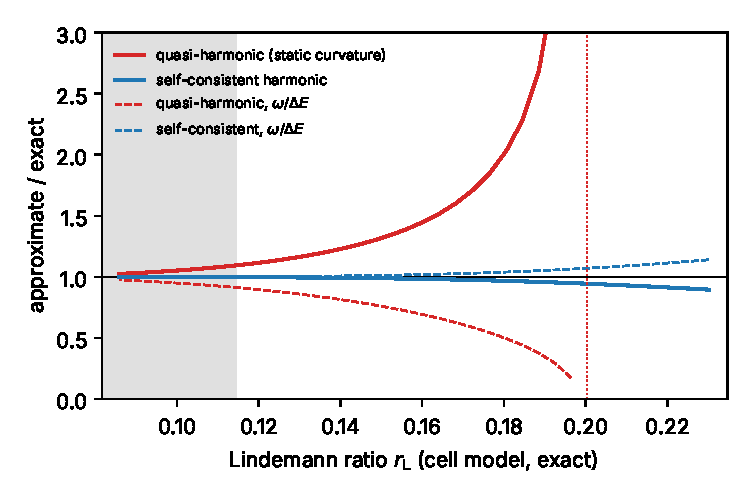
\includegraphics[width=\linewidth]{figures/ch11/limit11_5b.pdf}
\captionof{figure}{Cell model of solid $^4$He: one atom in the spherically averaged field of 12 fixed fcc neighbors, Morse pair potential with the well depth \SI{10.8}{K} and position \SI{2.967}{\angstrom} of the Aziz potential and a curvature equal to that of a 12-6 potential with the same well. Solid: one-phonon weight per unit $q^2$, $1/2M\omega$, from the static curvature (red, quasi-harmonic) and from the self-consistent curvature (blue), divided by the exact dipole weight of the lowest $l = 1$ level, against the exact Lindemann ratio $r_{\mathrm{L}}$, for molar volumes from 3 to \SI{21}{cm^3.mol^{-1}}. Dashed: the corresponding phonon energies over the exact excitation energy $\Delta E$. Dotted: $r_{\mathrm{L}} = 0.20$, above which the static curvature is negative. Gray band: $r_{\mathrm{L}} \le 0.115$, where the quasi-harmonic weight is within \SI{10}{\percent}.}\label{fig:11-limit-5b}
\par}
\smallskip
Above a Lindemann ratio of about 0.12 the static Hessian overstates the one-phonon weight and the Debye--Waller exponent, and above 0.20 it has no real frequencies; the self-consistent phonons hold to near melting, where correlations at short range remain.
\end{limitbox}

\noindent The model fixes the neighbors and uses a Morse wall, so its numbers are a guide, not a prediction for helium; it lands within $0.003$ and $0.006$ of the two Monte Carlo ratios. The quasi-harmonic response of Ashour and Griffin is safe in most of their pressure range and needs the self-consistent force constants at its low end. And at the lowest pressures, where a helium detector would be easiest to build, neither is exact. The self-consistent weight is \SI{10}{\percent} low near melting even in the model, and in the real crystal the Gaussian lets an atom overlap its neighbors, which a real atom avoids by correlated motion. There the response needs the exact moments and the band of \cref{lim:11.5c}. On the truncation label the self-consistent response sums the even anharmonic orders into $\Phi^{(2)}_{\mathrm{aux}}$ at all $n_A$. The cubic terms enter the physical frequencies through a bubble; in the cubic cell of the model the centroid sits on the site and that bubble vanishes.

The same reasoning sorts the other targets in which anharmonicity is not small. A soft mode, such as the one that drives the structural transition of SrTiO$_3$, has a harmonic frequency that is small or imaginary, and its self-consistent frequency depends on temperature at order one. A light atom, such as hydrogen in LiH, has a zero-point amplitude larger by $(M_{\mathrm{Si}}/M_{\mathrm{H}})^{1/4} \approx 2.3$ than a silicon atom in the same well, since $\ell_{\mathrm{zp}} \propto M^{-1/4}$ (\cref{sec:5.7}), and $\eta_{\mathrm{anh}}$ grows with it.

\emph{Open problem: the response of strongly anharmonic targets at detector temperatures.} For soft-mode and light-atom crystals, and for solid helium near melting, no expansion parameter is small, and the nuclear response at \SI{10}{mK} has not been computed. The exact moments are within reach: they are static averages, and a path-integral simulation gives them at any temperature and anharmonicity. The dynamics is not. Ring-polymer and centroid molecular dynamics return Kubo-transformed correlations. Their conversion to $S$ multiplies the error by $\omega/T$, so they hold only for $T \gtrsim \omega/10$; the time-dependent self-consistent harmonic method excites at most two phonons at a time and cannot follow a multiphonon response at $q \gg q_{\mathrm{BZ}}$. At the operating temperature of a cryogenic detector the response of these targets is therefore bounded by the band of their exact moments and by nothing sharper. What would close the gap is a real-time method for quantum nuclei that is exact at low temperature, or a measurement: neutron Compton scattering measures the momentum distribution, and with it the impulse width, of light nuclei directly~\cite{andreani2005measurement}.
